\documentclass[11pt]{article}
\usepackage{fontspec}
% \usepackage[T1]{fontenc}	%special characters
% \usepackage[utf8]{inputenc}	%special characters

\usepackage{lmodern,textcomp}% Euro Symbol
\usepackage[a4paper, top=0.5in, right=0.5in, bottom=0.5in, left=0.5in]{geometry} %article layout margins
\usepackage{hyperref}


\usepackage{tabularx}		%tabulars width fixed textwidth
\usepackage{multicol}	%2 columns in Skills
\usepackage{multirow}
\usepackage{graphicx}
\usepackage{tikz}
\usetikzlibrary{shapes.geometric,calc}
\usepackage{xcolor}

\setlength\parindent{0pt}
\renewcommand\tabularxcolumn[1]{m{#1}}% for vertical centering text in X column

\definecolor{lightgray}{rgb}{239,239,239}
% \definecolor{maincolor}{RGB}{0,180,230}
\definecolor{maincolor}{RGB}{0,112,243}

\newcommand\score[2]{
\pgfmathsetmacro\pgfxa{#1+1}
\tikzstyle{scorestars}=[circle, inner sep=0.2em,anchor=west]
\begin{tikzpicture}[baseline]
  \foreach \i in {1,...,#2} {
    \pgfmathparse{(\i<=#1?"maincolor":"lightgray")}
    \edef\starcolor{\pgfmathresult}
    \draw (\i*1.5em,0.25em) node[name=star\i,scorestars,fill=\starcolor]  {};
   }
  \pgfmathparse{(#1>int(#1)?int(#1+1):0}
  \let\partstar=\pgfmathresult
  \ifnum\partstar>0
    \pgfmathsetmacro\starpart{#1-(int(#1))}
    \path [clip] (star\partstar.north west) rectangle 
    ($(star\partstar.south west)!\starpart!(star\partstar.south east)$);
    \fill (\partstar*1em,0) node[scorestars,fill=blue!70]  {};
  \fi,

\end{tikzpicture}
}
\newcommand\skill[1]{
 \begin{tikzpicture}
   \fill [white] (0,0) rectangle (\linewidth,.2);
   \fill [maincolor] (0,0) rectangle (#1 \linewidth,.2);
 \end{tikzpicture} 
}
\newfontfamily\unicodefont{Lucida Grande}
\setmainfont{HK Grotesk}
\pagenumbering{gobble}

% Project List
\newcommand{\minitab}[2][l]{\begin{tabular}{#1}#2\end{tabular}}
\newcolumntype{P}[1]{>{\centering\arraybackslash}p{#1}}
% Tags
\usepackage{tcolorbox}
\newtcbox{\tagBox}{on line,
  colback=maincolor,
  boxrule=0pt,arc=5pt,boxsep=1pt,left=0pt,right=0pt,top=2pt,bottom=2pt}
\newcommand{\tag}[1]{\footnotesize\tagBox{\color{white}{\phantom{g}#1\phantom{g}}}}


\begin{document}

\begin{minipage}[t]{0.25\textwidth}
\section*{Dirk Hornung, PhD}

\vspace{0.8cm}

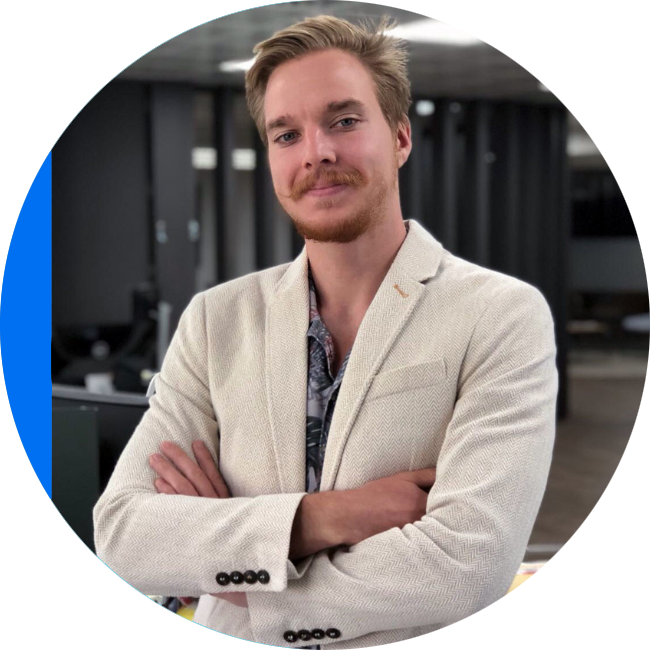
\includegraphics[width=\linewidth]{dirkRound.png}

\vspace{1.1cm}

\begin{footnotesize}
\begin{tabularx}{\linewidth}{@{}>{\bfseries}ll@{}}
City:       & Barcelona \\
Birthdate:  & October 5, 1991\\
Birthplace: & Fulda, Germany \\
Mobile:     & +34 695460404 \\
E-mail:     & hello@drdirk.io \\
Website:    & https://drdirk.io
\end{tabularx}
\end{footnotesize}

\vspace{0.5cm}

\small
\subsection*{Languages}
\begin{tabularx}{\linewidth}{@{}Xc @{}}
German & \score{5}{5} \\
English & \score{4}{5} \\
French & \score{3}{5} \\
Spanish & \score{4}{5} 
\end{tabularx}

\vspace{0.7cm}

\subsection*{Skills}

\begin{tabularx}{\linewidth}{@{}lX @{}}
  Data Science & \skill{0.6} \\
  Frontend & \skill{.9} \\
  Backend & \skill{.8} \\
  Blockchain & \skill{.4} \\ 
  Prototyping & \skill{.2}
\end{tabularx}

\vspace{1.5cm}

\footnotesize
\textbf{Data Science}\\
Python, Tensorflow, Keras, Hadoop, 
Pandas, Numpy, Matplotlib, Deep Learning \\
\textbf{Frontend}\\
JavaScript, TypeScript, React, Angular, React Native, Redux,
Flutter, Jasmine, Mocha, CSS, HTML \\
\textbf{Backend}\\
AWS, NodeJS, Express, MySQL, PostgreSQL, MongoDB, DynamoDB,
Serverless, Flask, Docker, Kubernetes \\
\textbf{Blockchain}\\
Ethereum, Solidity, Smart
Contracts, Hyperledger Fabric, Token Economy, ICO \\
\textbf{Prototyping} \\
Arduino, C++, Fusion 360, 3D-Printing, CNC, Electronics

\end{minipage}
\hspace{0.05\textwidth}
\begin{minipage}[t]{0.65\textwidth}


\section*{Professional Experience}
\begin{tabularx}{\textwidth}{lX}
  \small 05/18 - 02/19 & \textbf{CYSAE} - Legaltech Startup\\
                & \textit{CTO} (2 Developers) \\
                & \small \textbf{Utility Token for Cuatre Casas} \\
                & \small Created an Utility Token, within the Ethereum Blockchain, that allows to buy legal services by
                  paying with a Cryptocurrency. \\
                  % & Customised an ERC-20 Solidity Smart Contract for
                  %   a Spanish lawyer agency. Configured and launched an
                  %   Ethereum Node connected to a Node-Express REST API to consume
                  %   the token functionality. \\[1.5mm]
                & \small \textbf{Stamper} \\
                & \small Created a web application that anchors documents in the Ethereum
                  Blockchain, to establish secure contracts.\\
                  % Developed a React-Redux Web App with an
                  % GraphQL-Prisma-MySQL backend hosted on AWS-ERC docker
                  % containers and AWS-S3. \\[1.5mm]
                & \small \textbf{Boardchain} \\
                & \small Developped a web application to remotly hold decentralised
                  board meetings. \\\\
                  % & Developed a DAO to decentralise board meetings. The
                  %   Web App was based on React-Redux backed by
                  %   Serverless AWS-Lambda, AWS-S3, AWS-Cognito and AWS-Dynamodb. \\\\
  \small 10/17 - 04/18 & \textbf{Alda} - Fintech Startup\\
                & \textit{CTO \& Co-Founder} (1 Developer) \\
                & \small \textbf{Alda Chatbot} \\
                & \small Created a Fintech Chatbot that serves as a personal financial
                  advisor.\\
                  % & Created a Fintech Chatbot Modelled and
                  % trained a RNN before switching to the Dialogflow API
                  % for the NLP. Created a Serverless Python-Flask-AWS-RDS (PostgreSQL) backend,
                  % combining the Facebook and Saltedge API to connect
                  % and query financial information of our clients. \\[1.5mm]
                & \small \textbf{Chatbot UI} \\
                & \small Created a mobile app for the Chatbot, which has been
                  integrated in several companies.
                  % & Created React-Redux PWA connected to our chatbot.
                  % Integrated the app in various Wordpress and Liferay
                  % installations. \\\\
\end{tabularx}

\vspace{0.3cm}

\section*{Education}
\begin{small}
\begin{tabularx}{\textwidth}{lX}
  % 2019        & \textbf{Deep Learning Specialisation} \\
  %             & Absolved five classes of the Coursera specialisation of Deep Learning to study Neural Networks,
  %               Hyperparameter tuning, Machine Learning projects, Convolutional Neural Networks and Sequence Models. \\\\
  10/15 - 07/19 & \textbf{Ph.D., Theoretical Physics}, UAB (Spain) / AMU (France) \\
                & Thesis: The QCD Strong Coupling from Hadronic Tau
                  Decays \\\\
  10/14 - 09/15 & \textbf{M.Sc., Particle Physics}, UAB (Spain) \\
                & Thesis: 1-Loop Anomalous Dimensions of 4-Quark
                  Operators \\\\
  10/11 - 09/14 & \textbf{B.Sc., Condensed Matter Physics}, GU (Germany) \\
                & Thesis: Band Structure Studies of Graphene and Modified
                  Graphene Structure
\end{tabularx}
\end{small}

\vspace{0.3cm}

\begin{small}
\section*{Awards}
\begin{itemize}
\item \textbf{Imagine Silicon Valley Finalist}. \\
One of ten finalists of more than 500 applicants to be sponsored for a Silicon Valley trip.
\item \textbf{Winner: Imagine Developer Dreamer}. \\
 Got selected to participate in the "Imagine-Express-Train".
\item \textbf{Best Fintech Pitch} \\
Awarded 1st price at Fintech Stage's event ``Fintech War'' of over
+16 fintech startups plus a 1k€ cash price
\item \textbf{Winner Adidas Finals Hackathon} \\
Created the ``Adidasum'' ICO for an API data marketplace.
\item \textbf{MetLife Iberia Financial Inclusion Award} \\
Awarded a 4K€ cash price at MetLife Iberia to keep
promoting Financial Inclusion.
\item \textbf{Winner Adidas Hackathon Barcelona} \\
Created surveillance system to track and identify customer satisfaction.
\end{itemize}
\end{small}
\end{minipage}

\section*{Projects}
\begin{tabularx}{\linewidth}{p{0.15\linewidth}p{0.15\linewidth}p{0.65\linewidth}}
  12/19 - presend &
  \multirow[t]{2}*{\minitab{ \\ \textbf{1++ App} \\ Front-End}} 
  & Created an Angular Ionic Hybrid App connected to   Firebase. Designed NoSQL
    database architecture. Used RxJS Observables. Used TDD with Jasmine and
    Karma.\\
  && \tag{JavaScript} \tag{Angular 8} \tag{Ionic} \tag{RxJS} \tag{Firebase}
     \tag{Jasmine} \tag{Material Design} \\\\

  10/18 - 02/19 &
  \multirow[t]{2}*{\minitab{ \\ \textbf{Utility Token} \\ Blockchain}} 
  & Created an Ethereum ERC-20 compliant utility token for Cuatre Casas. Created
  a Node-Express REST API connected to an Ethereum Node to manage Token
    interactions. Used Truffle and Mocha for Unit-testing.\\
  && \tag{JavasScript} \tag{Node} \tag{Express} \tag{REST} \tag{Mocha} \tag{Ethereum} \tag{Solidity} \tag{Truffle} \\\\

  04/18 - 11/18 &
  \multirow[t]{2}*{\minitab{ \\ \textbf{Stamper} \\ Full-Stack}} 
  & Created an React-Redux App with an Prisma-GraphQL backend hosted on AWS
    ECS. Used AWS Cognito for authentification and AWS S3 for storage.\\
  && \tag{React} \tag{Redux} \tag{JavaScript} \tag{Prisma} \tag{GraphQL} \tag{AWS-ECS} \tag{AWS-Cognito} \tag{AWS-S3} \\\\
  
  04/18 - 02/19 &
  \multirow[t]{2}*{\minitab{ \\ \textbf{Boardchain} \\ Blockchain}} 
  & Created an React-Redux App connected to a series of Smart Contracts hosted
    on the Ethereum Blockchain to remotely
    hold transparent and immutable board meetings.\\
  && \tag{React} \tag{Redux} \tag{JavaScript} \tag{Solidity} \tag{Ethereum} \tag{Smart Contract} \tag{Truffle} \\\\

  10/17 - 04/18 &
  \multirow[t]{2}*{\minitab{ \\ \textbf{Alda Chatbot} \\ Data Science}} 
  & Created an natural language processor to detect user intents. Connected the
    Facebook API, Saltedge API and Dialogflow API to create a Chatbot interface
    able to respond to many financial requests. Hosted serverless microservices
    as AWS Node and Python Lambdas with a PostgreSQL database as backend. \\
  && \tag{Data Science} \tag{NLP} \tag{AWS-Lambda} \tag{PostgreSQL} \tag{Python}
  \tag{JavaScript} \tag{Node} \tag{Serverless} \\\\

  10/17 - 04/18 &
  \multirow[t]{2}*{\minitab{ \\ \textbf{Alda PWA} \\ Front-End}} 
  & Created a React PWA for the Chatbot as UI alternative for Facebbook Messenger. \\
  && \tag{React} \tag{Redux} \tag{AWS-Amplify} \tag{AWS-Dynamodb} \tag{Serverless}
  \tag{AWS-Cognito} \\\\

  09/16 - 09/17 &
  \multirow[t]{2}*{\minitab{ \\ \textbf{WeGoLoco App} \\ Full-Stack}} 
  & Created a native iOS App written in Swift. Used AWS-Cognito for
    authentification, AWS-RDS (PostgreSQL) as a database and AWS-S3 for storage
    connected via AWS-Lambda Serverless microservices. \\
  && \tag{Native App} \tag{Swift} \tag{AWS-Cognito} \tag{AWS-RDS}
     \tag{AWS-Lambda} \tag{AWS-S3} \tag{PostgreSQL}\\\\

  02/16 - 08/16 &
  \multirow[t]{2}*{\minitab{ \\ \textbf{FuldaCity App} \\ Front-End}} 
  & Created a Native App written in React Native with a MongoDB backend. \\
  && \tag{React Native} \tag{JavaScript} \tag{MongoDB}\\\\

  01/16 - 06/15 &
  \multirow[t]{2}*{\minitab{ \\ \textbf{Tennisspot} \\ Full-Stack}} 
  & Created a Web App for a local tennisclub, which is still used by > 200
    Persons. Used LAMP with PHP and MySQL. \\
  && \tag{PHP} \tag{MySQL} \tag{JQuery} \tag{LAMP}\\\\
  

\end{tabularx}





	
% \section*{Professional Profile}
% Theoretical solid-state and high-energy physicist. \hfill 7+ years \\[1mm]
% Data Scientist \hfill 4+ years \\[1mm]
% Software Architect \hfill 2+ years \\[1mm]
% Blockchain Developer \hfill 2+ years \\[1mm]
% Full Stack Developer \hfill 10+ years \\[1mm]


% COVERLETTER %%%%%%%%%%%%%%%%%%%%%%%%%%%%%%%%%%%%%%%%%%%%%%%%%%%%%%%%%%%%%%%%%%
 % \section*{}
 % \vspace{1cm}
 % Dear , \\
 

 % \noindent I am Dirk Hornung, a recently graduated Ph.D. student at
 % the institute of high energy physics of the Autonomous University of
 % Barcelona with 5+ years of experience in leading the technology in
 % different Startups. Within my studies, I researched low-energy QCD
 % and the determination of Standard Model parameters. I developed a C++
 % fitting routine to extract parameters of
 % theoretical models out of CERN experimental data. \\

 % \noindent Besides my studies, I am an entrepreneur. During the last year, I
 % developed Smart Contracts in the Ethereum Blockchain and connected them through
 % REST APIs using Node Express for a legaltech. Before I developed a chatbot
 % using Artificial Intelligence for a fintech. We connected our clients through
 % Messenger to their bank accounts and analyzed their banking information using
 % Python. I am furthermore a Full-stack developer with lots of experience
 % developing applications using React as frontend and AWS services as a backend.  \\

 % \noindent Currently I am educating myself on the topic of Artificial Intelligence
 % and Machine Learning, especially in the field of Deep Learning. I recently completed
 % Andrew Ng's Coursera Deep Learning Specialization. Apart from that, I am practising my
 % Tensorflow and Keras skills within python sound wave simulations and active noise cancelling.\\


 % \noindent Sincerely, \\
 % Dr. Dirk Hornung \\

 % \noindent P.S. I love Tech and would be interested in a position as Technology Consultant.
 % \noindent P.S. I am a native German, but also fluent in English, French and
 % Spanish. Visit drdirk.io to get to know me better.
%%%%%%%%%%%%%%%%%%%%%%%%%%%%%%%%%%%%%%%%%%%%%%%%%%%%%%%%%%%%%%%%%%%%%%%%%%%%%%%%


% \section*{Professional Experience}
% \begin{tabularx}{\textwidth}{lX}
%   % since July 2019        & \textbf{Sharify} \\
%   %                        & \textbf{CTO \& Backend Developer} \\[2mm]
%   %                        & Scaling the backend of Sharify, a Startup connecting thousands of
%   %                        users on a live map. Architecting NoSQL databases and Node Microservices.\\\\
%   05/2018 - 02/2019   & \textbf{CYSAE} \\
%                          & \textit{CTO} (2 Developers) \\[2mm]
%                          & \textbf{Utility Token for Cuatre Casas} \\
%                          & Customised an ERC-20 Solidity Smart Contract for
%                            a Spanish lawyer agency. Configured and launched an
%                            Ethereum Node connected to a Node-Express REST API to consume
%                            the token functionality. \\[1.5mm]
%                          & \textbf{Stamper} \\
%                          & Developed a React-Redux Web App with an
%                            GraphQL-Prisma-MySQL backend hosted on AWS-ERC docker
%                            containers and AWS-S3. \\[1.5mm]
%                          & \textbf{Boardchain} \\
%                          & Developed a DAO to decentralise board meetings. The
%                            Web App was based on React-Redux backed by
%                            Serverless AWS-Lambda, AWS-S3, AWS-Cognito and AWS-Dynamodb. \\\\
%   10/2017 - 04/2018  & \textbf{Alda} \\
%                          & \textit{CTO \& Co-Founder} (1 Developer) \\[2mm]
%                          & \textbf{Alda Chatbot} \\
%                          & Created a Messenger Fintech Chatbot. Modelled and
%                            trained a RNN before switching to the Dialogflow API
%                            for the NLP. Created a Serverless Python-Flask-AWS-RDS (PostgreSQL) backend,
%                            combining the Facebook and Saltedge API to connect
%                            and query financial information of our clients. \\[1.5mm]
%                          & \textbf{Chatbot UI} \\
%                          & Created React-Redux PWA connected to our chatbot.
%                            Integrated the app in various Wordpress and Liferay
%                            installations. \\\\
% %  Feb. 2017 - Sept. 2017 & \textbf{WeGoLoco} \\
% %                         & \textit{CTO \& Co-Founder} \\[1mm]
% %                         & Created a native iOS app based on Swift. \\

%   %                          2017 & \textbf{FuldaCity} \\
%   %                          & \textit{CTO \& Co-Founder} \\[1mm]
%   %                          & Bringing my Hometown online within the
%   %                          Meteor/React Framework \\[1mm]
%   %                          & http://www.fuldacity.de/ \\\\
  
%   %              %                          \pagebreak
  
  
  
%   %                          2013 - 2016 & \textbf{Fulda Strategy Group GbR -
%   %                          Management Consultancy} \\
%   %                          & \textit{Founder and Managing Director} \\[1mm]
%   %                          & Projects in the area of ERP selection and
%   %                          implementation, process management and software
%   %                          development \\[1mm]
%   %                          & www.fulda-strategy.com \\\\
  
%   %                          2010 - present & \textbf{Eevents Fulda GbR -
%   %                          Event Management} \\
%   %                          & \textit{Founder} \\[1mm]
%   %                          & Organising of company events, weddings and
%   %                          birthdays \\[1mm]
%   %                          & www.eevents-fulda.de \\\\
  
%   %                          2010 - 2014 & \textbf{Hornung Webdesign -
%   %                          Webdesign Agency} \\
%   %                          & \textit{Founder} \\[1mm]
%   %                          & Developing and maintaining of CMS and SaaS.
%   %                          \\\\
% \end{tabularx}


		
% \section*{Skills}
% \begin{tabularx}{\textwidth}{lX}
%   \textbf{Data Science} & Python, Tensorflow, Keras, Hadoop,
%                           Spark, Pandas, Numpy, Matplotlib, SVM,
%                           NN, CNN, RNN
%                           Mathematica \\
%   \textbf{Frontend}     & JavaScript, React, React Native, Redux, Flutter, CSS, HTML  \\
%   \textbf{Backend}      & AWS, Node, Express, MySQL, PostgreSQL, DynamoDB,
%                           Serverless, Flask, Zappa, Django \\
%   \textbf{Blockchain}   & Ethereum, Solidity, Smart Contracts,
%                           Tokens economy,
%                           Decentralised Identity, ICOs \\
%   \textbf{Prototyping}  & Arduino, C++, Fusion 360, 3D-Printing,
%                           CNC, Electronics \\
%   \textbf{Marketing}    & Photoshop, Illustrator, Final Cut Pro, SEO, SEM, Wordpress, PHP \\
%   \textbf{Soft}         & Leadership, Public Speaking, Motivating, Mentoring, Confidence, Energy
% \end{tabularx}

% \section*{Awards}
% \begin{tabularx}{\textwidth}{lX}
%   07/2019      & \textbf{Imagine Silicon Valley Finalist}. \\
%                  &  One of ten finalists of more than 500 applicants who sent in a one minute
%                    video (https://www.youtube.com/watch?v=Om1DGAa7Cgw) to be sponsored for a Silicon Valley trip. \\\\
%   02/2018  & \textbf{Winner: Imagine Developer Dreamer}. \\
%                  &  Got selected to participate in the "Imagine-Express-Train". \\\\
%   09/2018 & \textbf{Best Fintech Pitch} \\
%                  & Awarded 1st price at Fintech Stage's event ``Fintech War'' of over
%                    +16 fintech startups plus a 1k€ cash price \\\\
%   07/2018      & \textbf{Winner Adidas Finals Herzogen-Aurach} \\
%                  &  Created the ``Adidasum'' ICO for an API data marketplace to
%                    democratise data and connect data provider, data scientists and
%                    data consumer.\\\\
%   05/2018       & \textbf{MetLife Iberia Financial Inclusion Award} \\
%                  & Awarded a 4K€ cash price at MetLife Iberia to keep
%                    promoting Financial Inclusion. \\\\
%   04/2018     & \textbf{Winner Adidas Hackathon Barcelona} \\
%                  & Created a system that could uniquely identify faces and track
%                    emotions. We trained a model to predict the probability of a
%                    client purchasing a certain item in an Adidas store.
% \end{tabularx}
		


% \section*{Funding}
% \begin{tabularx}{\textwidth}{sX}
%  2015 - present & Ph.D. PIF grant at the Autònoma de Barcelona (Spain), 1200
	% \euro / month
	% \end{tabularx}


	% \section*{Teaching Experience}
	% 	\begin{tabularx}{\textwidth}{sX}
	% 		2015 - 2018 & Universitat Autònoma de Barcelona, Theoretical Mechanics/
  %   Quantum Mechanics I/ Quantum Mechanics II, Complex Numbers/
  %   Teaching Assistant (Spanish) \\[1mm]
	% 		\centering{2014} & Goethe Universität Frankfurt, Quantum Mechanics I , exercise tutor \\
	% 		& Goethe Universität Frankfurt, Math for Physicists II, exercise tutor \\[1mm]
	% 		2013 - 2014 & Goethe Universität Frankfurt, Math for Physicists I, exercise tutor
	% 		% 	% \end{tabularx}


	% \section*{Publications}
	% 	\begin{tabularx}{\textwidth}{sX}
	% 		2015 & Diogo Boito, \textbf{Dirk Hornung}, Matthias Jamin \\[1mm]
	% 		& "Anomalous dimensions of four-quark operators and renormalon structure of mesonic two-point correlators" \\[2mm]
	% 		&  \textit{arXiv:1510.03812 [hep-ph]}	
	% 	\end{tabularx}


	% \section*{Oral presentations}
	% 	\begin{tabularx}{\textwidth}{sX}
  %    2018 & Aix Marseille Université, ``Determination of the QCD Coupling
  %    from
  %    ALEPH $\tau$-Decay data''
	% 	\end{tabularx}\vspace{1mm}
	% 	\begin{tabularx}{\textwidth}{sX}
	% 	2015 & Universitat Autònoma de Barcelona, Master Thesis Defence of : \\ & ``1-Loop anomalous dimensions of 4-quark operators''
	% 	\end{tabularx}\vspace{1mm}
	% 	\begin{tabularx}{\textwidth}{sX}
	% 		2014 & Goethe Universität Frankfurt, Group Seminar Talk: ``Band structure studies of Graphene and modified Graphene structures''
	% 	\end{tabularx}

	

%  \section*{References}
%	\begin{tabularx}{0.5\textwidth}{@{}l}
%		Prof. Dr. Roser Valentí \\
%		valenti@itp.uni-frankfurt.de \\
%		+49 69 798 47816 \\
%		Institut für Theoretische Physik \\
% 		Goethe-Universität Frankfurt am Main \\
% 		Max-von-Laue-Strasse 1 \\
%		60438 Frankfurt am Main \\
%		Germany 	
%	\end{tabularx}
%	\begin{tabularx}{0.5\textwidth}{ll}
%		Prof. Dr. Matthias Jamin \\
%		jamin@ifae.es \\
%		Institut de Fisica d'Altes Energies (IFAE) \\
%                Universitat Autònoma de Barcelona \\
%                Plaça Cívica \\
%                08193 Cerdanyola \\
%		Spain \\
%		\\
%	\end{tabularx}
	


\end{document}

% LocalWords:  io lX textwidth tabulars sX Adidasum Ph PIF renormalon ph save
% LocalWords:  für Theoretische Physik von Strasse Fisica d'Altes Plaça Cívica
% LocalWords:  Cerdanyola LocalWords

% Local Variables:
% TeX-engine: luatex
% End:
